\documentclass[12pt,a4paper, titlepage]{article}
\usepackage{amsmath}
\usepackage{graphicx}
\usepackage{float}
\usepackage{wrapfig}
\usepackage[russian]{babel}
\usepackage[utf8]{inputenc}


\title{Лабораторная работа 4. Методы решения уравнения переноса. Вариант 2, задание 9}
\date{2021\\Апрель}
\author{Петраков Иван\\\ МФТИ\\\\\\\\\\\\\\\\\\\\}
\hoffset = 0pt
\voffset = 0pt
\textheight = 700pt
\topmargin = 0pt
\headheight = 0pt
\headsep = 0pt
\marginparwidth = 0pt
\oddsidemargin = 0pt
\textwidth = 450pt

\begin{document}

\maketitle

\subsection*{Описание задачи}
\noindent\rule{\textwidth}{1pt}
Описание задачи представлено на рисунке 1:
\begin{figure}[H]
	\centering
	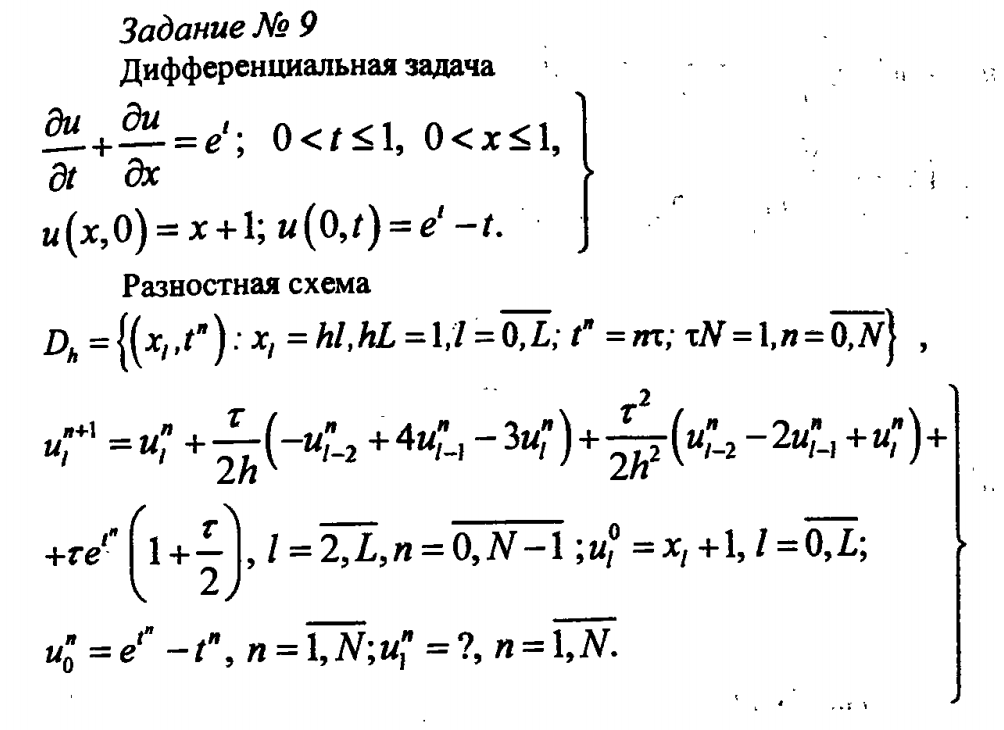
\includegraphics[width = 1.0\textwidth]{lab4_1.png}
\end{figure}

\subsection*{Аналитическое решение}
\noindent\rule{\textwidth}{1pt}



\subsection*{Программная реализация и практические исследования}
\noindent\rule{\textwidth}{1pt}

\subsection*{Результаты и обсуждения}
\noindent\rule{\textwidth}{1pt}
В данной работе найдено аналитическое решение поставленной задачи; разностная схема исследована на аппроксимацию, причем порядок аппроксимации, полученный из теоретических соображений и программно, одинаков; разностная схема исследована на устойчивость. Также найдены дополнительные условия, позволяющие детерминировать задачу. Были проведены практические исследования на основе программной реализации решения задачи, используя высокоуровневый язык программирования - Julia.

\end{document}